\section{Projektinitialisierung}\label{sec:Projektinitialisierung}

Der Rahmen des Projekts... 

\subsection{Unternehmen}

Über uns...


\subsection{Projekt}

\textit{Was ist das für ein Projekt? Was soll es bringen? }

Die freiwillige Feuerwehr von Eschenstruth gibt Feuerwehrkleidung für anliegende Ortsteile an Kinder aus. Dies gestaltet sich zunehmend schwerer, da die aktuelle Bestandspflege und der Überblick über die ausgegebene Kleidung mit den aktuellen Methoden schwer fällt. Vor wenigen Jahren wurden die Ausgabe und Verwaltung der Kleidung noch mit Zetteln dokumentiert. Dabei kam es durch uneinheitliches Vorgehen zu Verlust von Informationen. Dies geschah \zb durch den Verlust eines Zettels. Ein Zettel konnte schnell geschrieben, musste aber auch ordentlich in die entsprechende Akte eingepflegt werden. Zudem musste der Ort der Akte erst aufgesucht werden um das Schriftstück ab zuheften. 
Aktuell wird eine Excel"=Tabelle gepflegt. Diese befindet sich auf einem lokalen Rechner und einem USB"=Stick zur Datensicherung. Hier besteht der Nachteil, dass ein Rechner, auf dem sich de Excel"=Tabelle befindet, aufgesucht werden muss, um den Kleidereingang oder "=ausgang aus dem Lager zu dokumentieren. Als Zwischenspeicher wird eine Tafel verwendet, die bei der Ausgabe oder Annahme von Kleidung gefüllt wird (s. Abbildung~\ref{fig:tafel}). Der Warenbestand kann dann von einem beliebigen Rechner aus übertragen und dokumentiert werden, unter der Voraussetzung, dass die Person die aktuelle Excel"=Tabelle besitzt. Es muss aber bei der Synchronisation der Dokumentation darauf geachtet werden, dass die Daten in chronologisch richtiger Reihenfolge aufbereitet werden. Das kann unter Umständen, wenn zwei Personen zur gleichen Zeit an der Tabelle gearbeitet haben, zu einem erheblichen Mehraufwand führen, wenn nicht direkt nachvollziehbar ist, wer als letztes die Tabelle gepflegt hat, oder auf welchen Stand sich die Excel"=Tabelle befindet. 

\begin{figure}[hbtp]
  \centering
  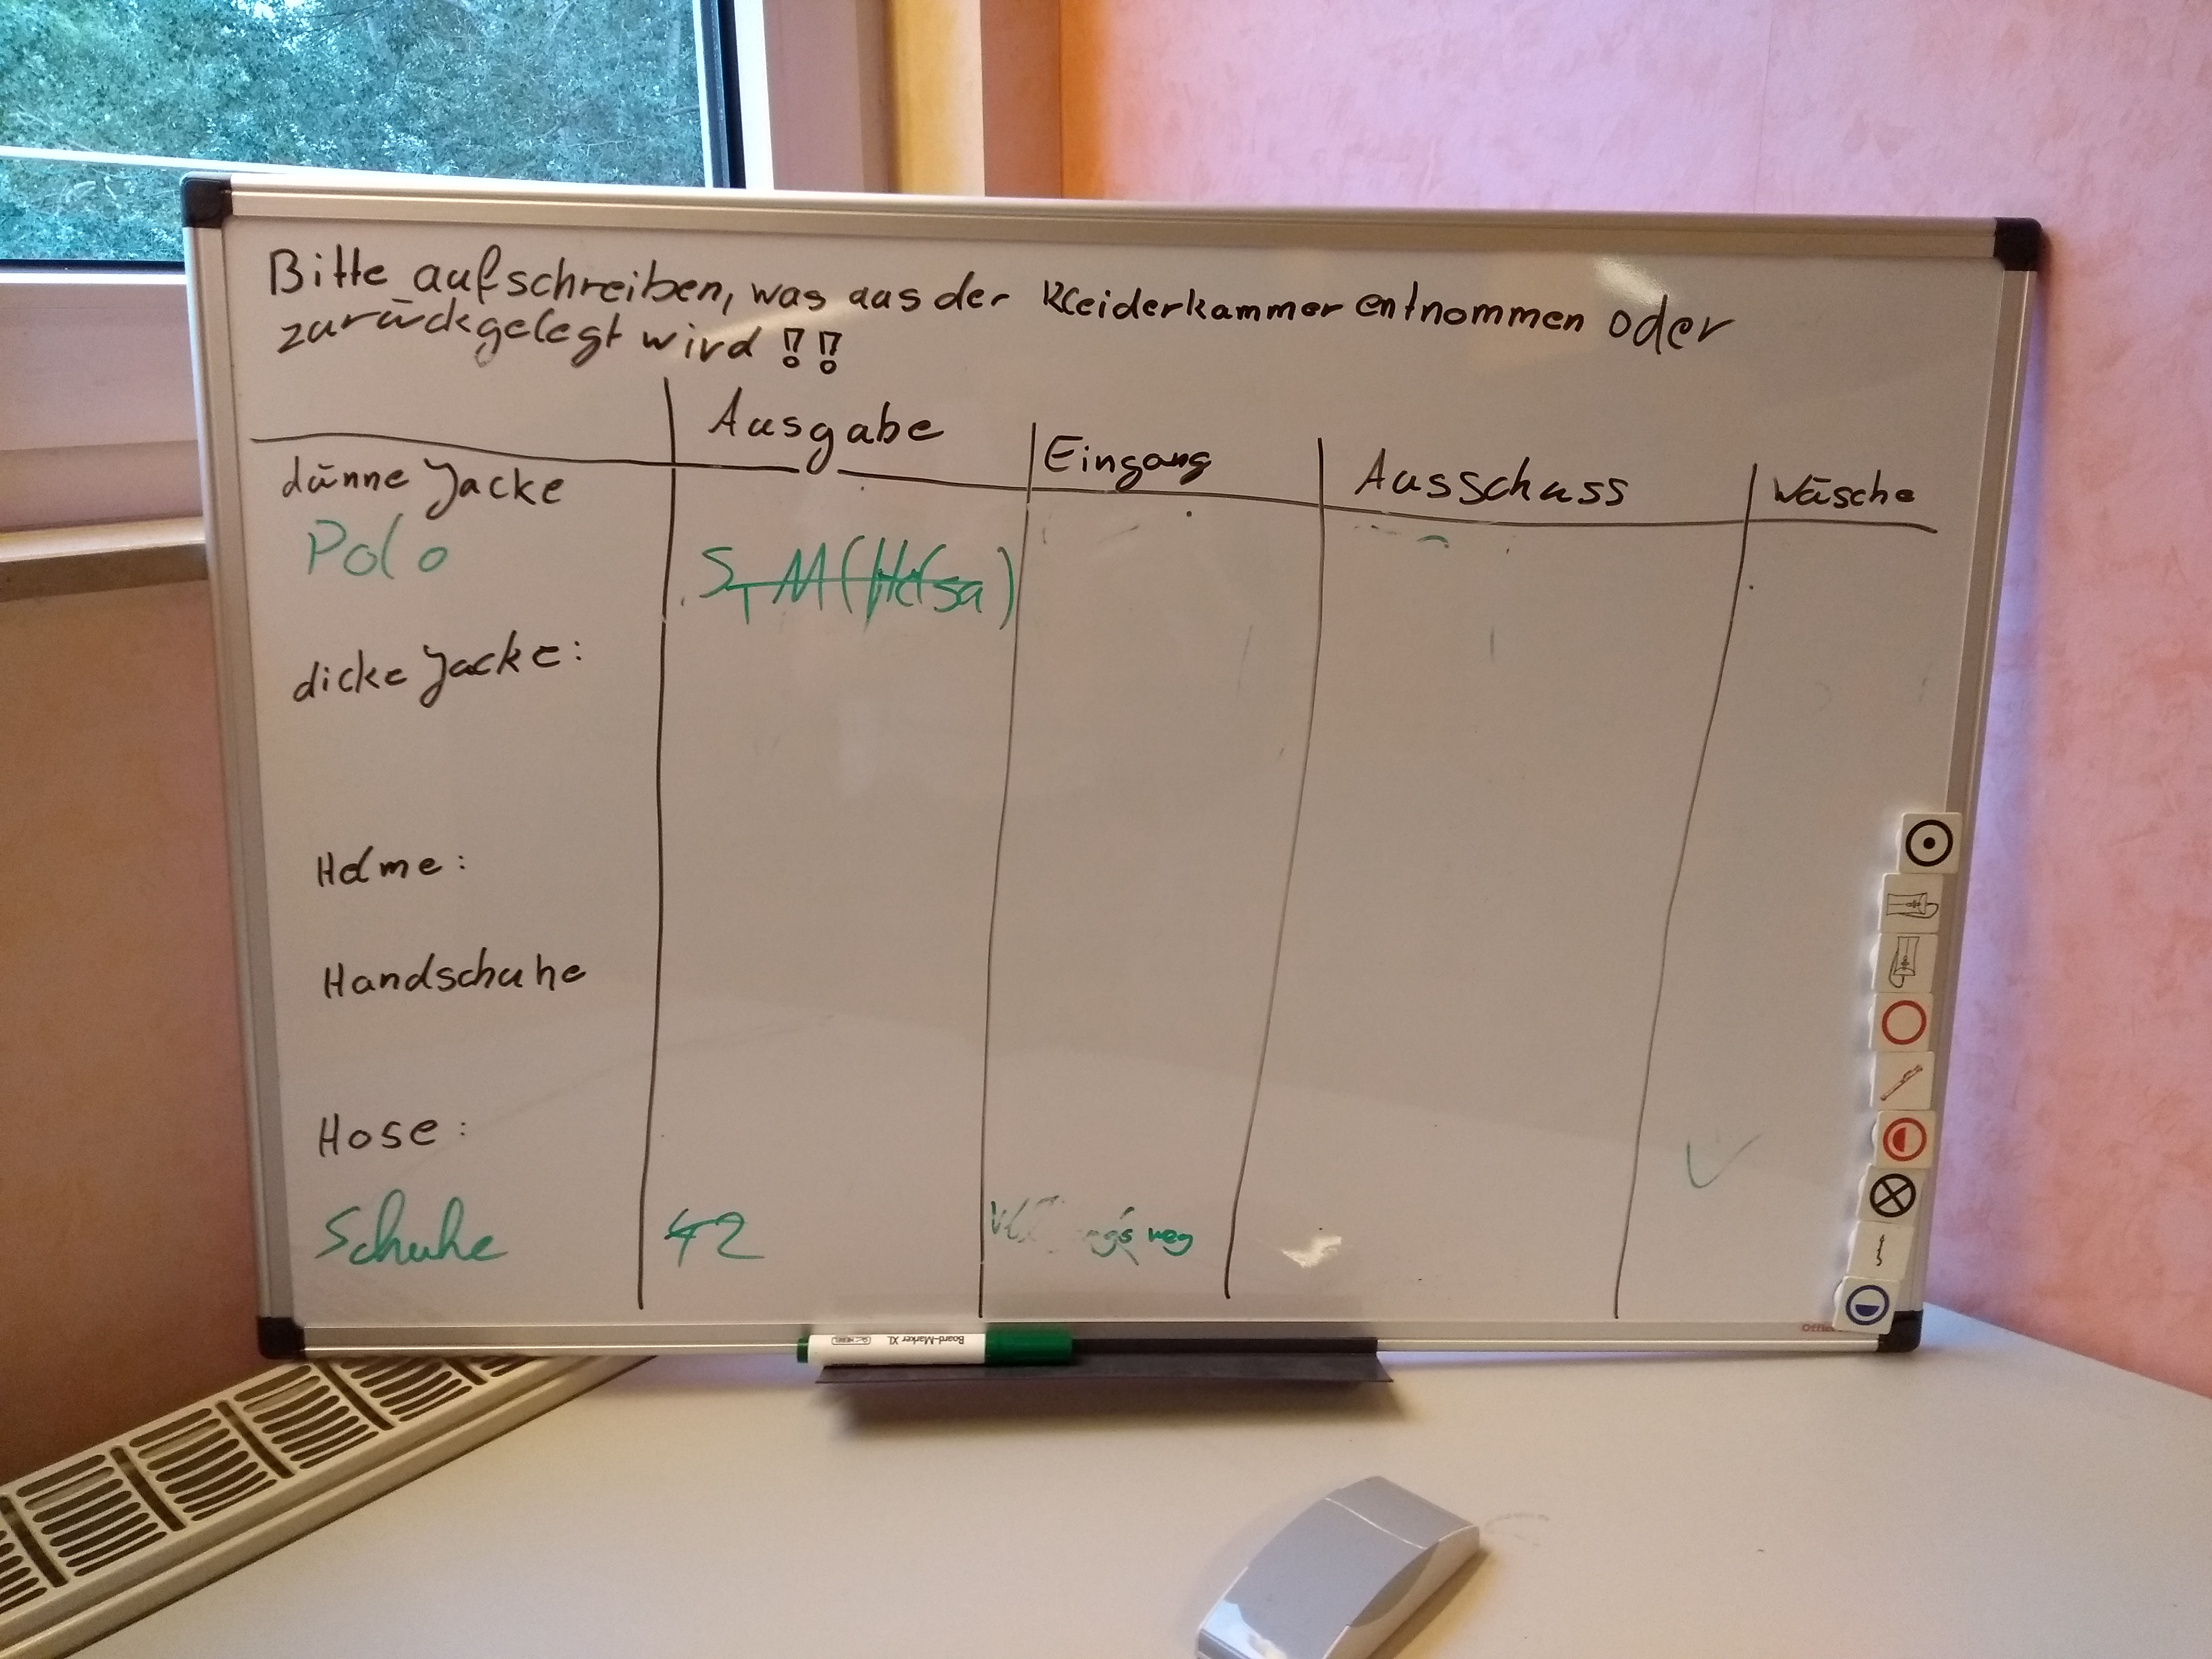
\includegraphics[width=0.95\textwidth]{res/IMG_20180815_193814370}
  \caption{Tafel aus Zwischenspeicher von Informationen.}
  \label{fig:tafel}
\end{figure}

Um die Probleme des Datenverlusts und der Synchronisation von Daten zu beseitigen, kam die Idee einer zentralen, aus dem Internet erreichbaren Kleiderverwaltung der Jugendfeuerwehr von Eschenstruth, oder auch \project.

In den folgenden Kapiteln werden die Kernziele dieses Projekts erläutert und die Erfolgskriterien definiert. Die beteiligten Personen an diesen Projekt werden erfasst und kurz vorgestellt. Darauf folgt der Projektansatz mit der Anforderungsspezifikation. Dabei werden alle Anforderungen die zwingend in diesem Projekt umgesetzt werden müssen definiert. 

\subsection{Project Definition Document}

\subsubsection{Gegenstand, Kernziele und Ziele des Projektes}

\textit{Welches Ziel wird damit verfolgt?}

Ziel ist es eine vollständig nachvollziehbare Dokumentation zu ermöglichen, bei dem zu jederzeit der aktuelle Aufenthaltsort der zur Verfügung stehenden Kleidung ermittelt werden kann. Dabei soll ein paralleles Arbeiten möglich sein. Die Anwendung muss auch von mobilen Geräten bedienbar sein, damit nicht nur ein Computer verwendet werden muss. Sie muss zudem intuitiv bedienbar sein. 

\subsubsection{Erfolgskriterien}

\textit{An was werden die Erfolgskriterien festgelegt?}

Ein Erfolgskriterium ist die vollständige Ablösung der Excel"=Tabelle und der Tafel. Die Daten werden nur noch über die Anwendung gepflegt.

\textit{Fällt uns nochwas ein? Bitte melden!!}


\subsubsection{Kontext des Projektes und die Projektabhängigkeiten}

\textit{In welchem Rahmen findet das Projekt statt?}

Das Projekt findet im Kontext des Studiengangs Sozialinformatik (B.Sc.) der Hochschule Fulda statt.

\subsubsection{Risiken, die den Projekterfolg verhindern könnten}

Was für Risiken können im Verlauf des Projekts auftreten?

Dadurch, dass das Projekt"=Team Vollzeit tätig ist, kann es zu Engpässen in der Durchführung kommen. Dies kann unter Umständen zu Mehrarbeit auf einzelne Team"=Mitglieder führen. Das Risiko ist gering einzuschätzen, da das Projekt"=Team  hinter der Idee steht.

Ein weiteres Risiko betrifft die Evaluation einer kostenlosen, bis kostengünstigen, Plattform, auf der die Anwendung bereit gestellt werden kann. Dabei kann die Akzeptanz der Endkunden sinken, wenn die Betriebskosten zu hoch ausfallen. Ab welchen Betrag die Kosten zu hoch sind, ist noch zu klären. Dieses Risiko ist mittelmäßig einzuschätzen, da es am Markt diverse Anbieter gibt. Unter den bekannteren Anbietern gehören \textit{AWS} vom \textit{Amazon} und \textit{Heroku}.

\subsubsection{Am Projekt Beteiligte}\label{sec:beteiligte}

Zum Projekt"=Team gehören:

\begin{itemize}
\item Tim Wieder, ist zuständig für den Kundenkontakt und die Frontend"=Entwicklung.
\item Achim Rose, ist zuständig für die Backend"=Entwicklung und den Entwurf der Datenbanktabellen. 
\item Sebastian Seeger, ist zuständig für die Infrastruktur. Das betrifft die Evaluation der Plattform und dessen Konfiguration.
\end{itemize}

Zu den Kunden gehören: 

\begin{itemize}
\item Nico M. (zuständig für die Kleiderkammer)
\item Julia W.
\item Marcel B.
\item Markus N.
\item Florian B.
\item Philipp H.
\end{itemize}

\subsubsection{Zu erwartender Projektansatz}

Wie wird das Projekt umgesetzt. Beschreibung der Vorgehensweise (agil und so)

\section{Projektplanung}\label{sec:Projektplanung}
\subsection{Anforderungsspezifikation}

Noch textlich verschriftlichen:

\begin{itemize}
\item Startseite
  \begin{itemize}
  \item Letzte Aktivitäten (Historisierung der Datenverarbeitung)
  \end{itemize}
\item System
  \begin{itemize}
  \item Benutzerverwaltung
    \begin{itemize}
    \item E-Mail Adresse
    \item Bestellt waren (an/aus) für Bestellung von neuer Kleidung
    \end{itemize}
  \item Steuerung, wer Klamotten aufnehmen kann, oder wer nur Daten lesen kann
  \item Ortsteilpflege 
    \begin{itemize}
    \item Ansprechpartner
    \item Warnungen bei Kleidungsart bei Ausgabe über eine bestimmte Stückzahl pro Ortsteil
    \end{itemize}
  \item Kleidungsarten verwalten.
  \end{itemize}
\item Aktionen / Übersicht
  \begin{itemize}
  \item Kleidung ausgeben (Hier auch mehrere Kleidungsstücke gleichzeitig)
    \begin{itemize}
    \item Art
    \item Größe
    \item Stückzahl
    \item An Ortsteil
    \end{itemize}
  \item Kleidung annehmen
    \begin{itemize}
    \item Lager (Wareneingang) / Ortsteil
    \end{itemize}
  \item Kleidung aussondern
    \begin{itemize}
    \item Lager / Ortsteil
    \end{itemize}
  \item Kleidung in Wäsche
  \end{itemize}
\item Auswertungen
  \begin{itemize}
  \item Filter über Kleidungsart, Zeitraum, Ausgaben nach Monaten/Jahren
  \item Größe
  \item Aber es soll auch eine Übersicht über alle Kleidungen geben
  \item Ausgesonderte Kleidungen
  \item Export nach Excel / ODF / PDF
  \end{itemize}
\item Warnmeldung bei geringer Stückzahl von Kleidung per Mail an den Verantwortlichen (Derjenige der die Kleidung bestellt.
\item Import einer aktuell verwendeten Exceltabelle
\end{itemize}


\subsection{Projektplan}
\subsubsection{Work-Breakdown-Structure}\label{sec:wbs}

Hier die Roadmap ausführlicher beschreiben als in GitHub.


\subsubsection{Ressourcenplanung}

Kann schon geplant werden, wer für welche Aufgabe zuständig ist? Dann eine Tabelle mit der Resourcenplanung erstellen.

\subsubsection{Zeitplanung}

Hier noch ein hübsches Gantt Diagramm? Oder einfach textlich auf die Roadmap verweisen?